\documentclass[12pt, letterpaper]{article}
\usepackage{hyperref}
\usepackage{graphicx}
%opening
\title{Wat2Search-SRP}
\author{rechstee, hudspero, lindo, milettal, sunamotl 
}

\begin{document}

\maketitle Project name: Wat2Search, Team:Team Chronic
	\\\underline{\textbf{User Interface Prototype:}}
	\\\\Home Screen:
	\\A widget on a webpage will open up to this home screen which displays the categories the non-technical user can choose from.  The user will identify a starting point in which they will determine the specific problem/issue they need help resolving.  The home screen will prompt the user to select the category pertinent to their case by physically “clicking” on a relevant box w/ the heading:
	
	Start from Category
	CLICK/SELECT:
	\\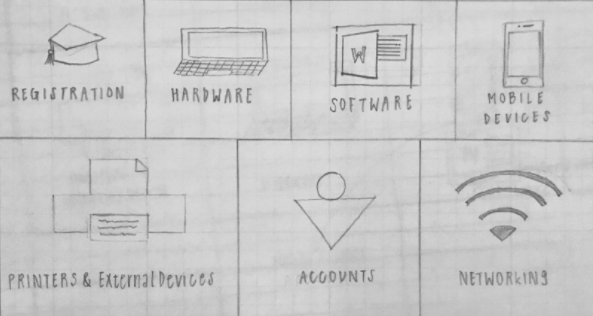
\includegraphics[scale=.75]{home.png}
	\\Following the user’s selection, the next screen will reflect the most common concerns that are within the chosen category.  This document includes sketches for our three chosen use cases: Networking (connecting to WiFi), Printers and External Devices (Printing Issues), and Accounts (reset Password)
	\\\\\textbf{Use Cases:}
	
\begin{enumerate}
	\item \textbf{Use Case 1:} Connecting to WiFi
	\\From: Start from Category
    \\NETWORKING
    \\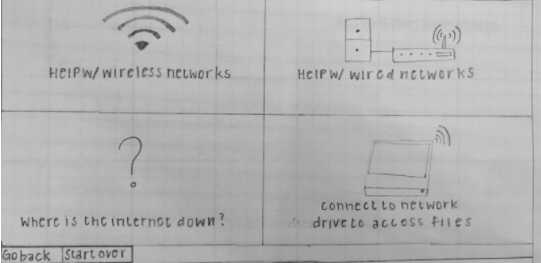
\includegraphics[scale=.75]{network.png}
    \\The above sketch illustrates the common concerns that the user can choose from.  Like the homepage, they will click on the relevant box to their concern.  This will hopefully help the user pinpoint their problem and receive the information they need more quickly.  They will also be continuously given the option of going back to the previous page or starting over at the homepage if their selection is not sufficient.  
    
    After clicking on one of the above options, they will be guided to specific option in which a set of instruction will be given for the user to resolve their concern/problem.
    \\From:NETWORKING
    \\Help w/ wireless networks
    \\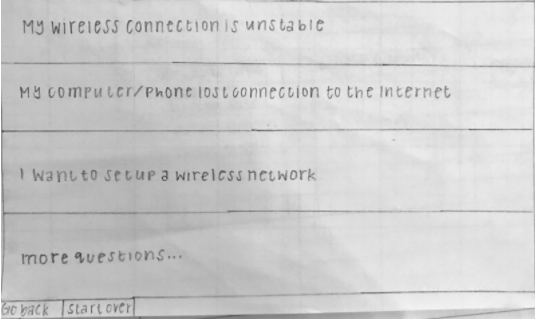
\includegraphics[scale=.75]{network_questions.png}
    
	\item \textbf{Use Case 2:} Resetting ONID Password
	\\From: Start from Category
	\\ACCOUNTS
	\\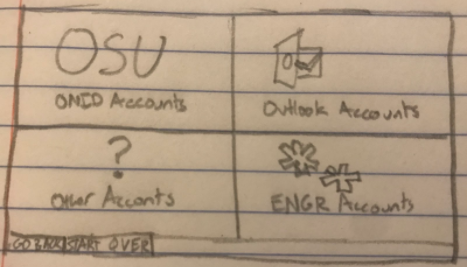
\includegraphics[scale=.75]{accounts.png}
	\\The above illustration shows the different options users can select after selecting the ACCOUNTS category from the home page. To access this page, a simple click on the square will take the user here. From here there are 4 different options: ONID accounts, Exchange accounts, ENGR accounts, and other accounts. Different icons were selected for each to help the user easily find what they are looking for. For this use case, the user would select the ONID accounts button leading them to the screen below.
	\\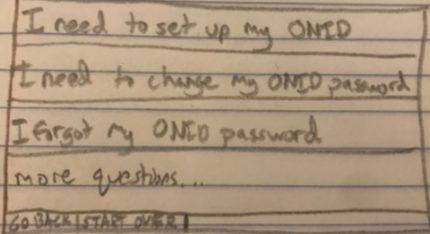
\includegraphics[scale=.75]{accounts_questions.png}	
	\\The screen above is the menu for when the user selects the ONID accounts from the Accounts menu. This category is broken up into specific questions that will guide the user to the correct solutions. Some of the questions that can be included for this is “I need to set up my ONID” or “I need to reset my ONID password”. The “more questions…” at the bottom of the diagram will be filled with any other questions we deem necessary to add. Not all are included now as this a constantly evolving prototype. 
	\\For this case study, the “I need to change my ONID password” would be selected. From here, the user would be taken to a screen with instructions on how to change their password. The screen would be setup with text and screenshots in the format shown below.
	\\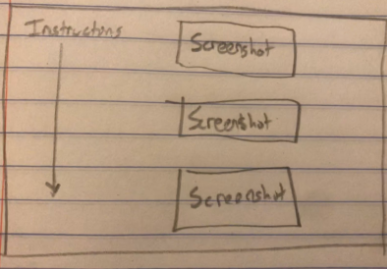
\includegraphics[scale=.75]{accounts_instructions.png}
	\item \textbf{Use Case 3:} On Campus Printer Malfunctioning
	\\From: Start from Category
	\\Printers and External Devices
	\\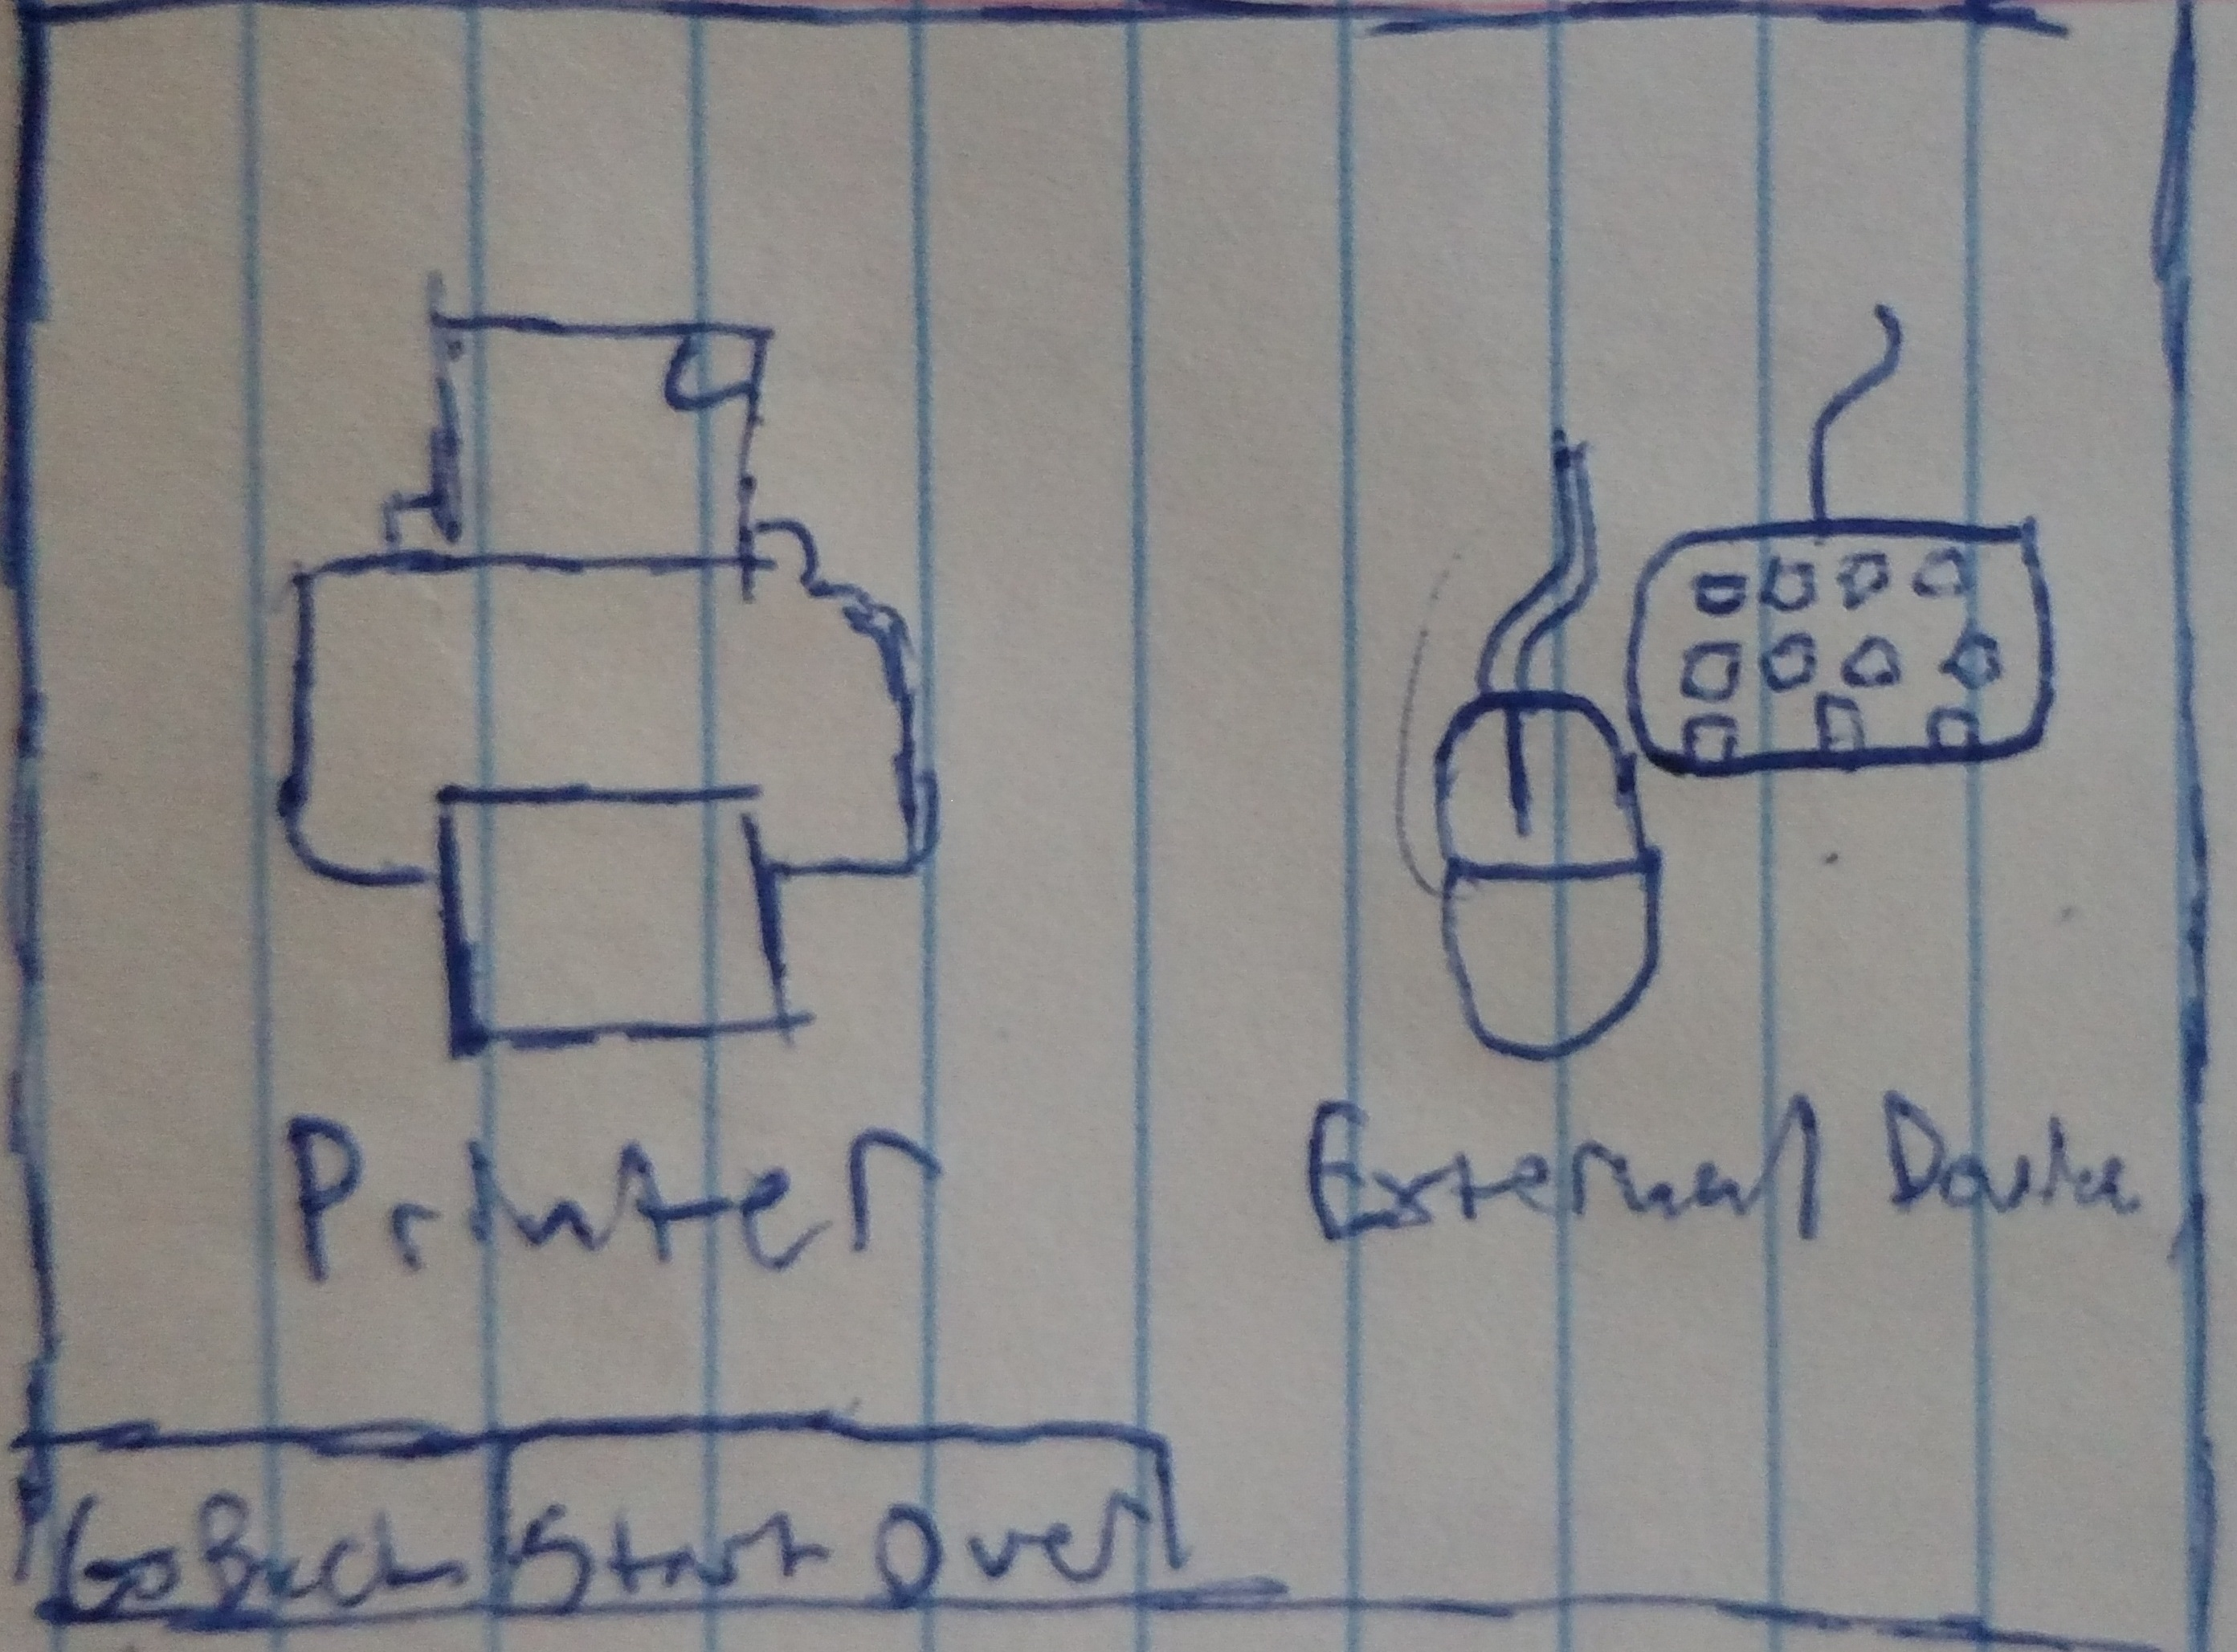
\includegraphics[scale=.075]{printer_etc.jpg}
	\\The above screen is after the user clicks the Printers and External Devices. It has the user choose whether they are using a printer or an external device like ,for instance, a mouse. In this use case, the choice is a printer.
	\\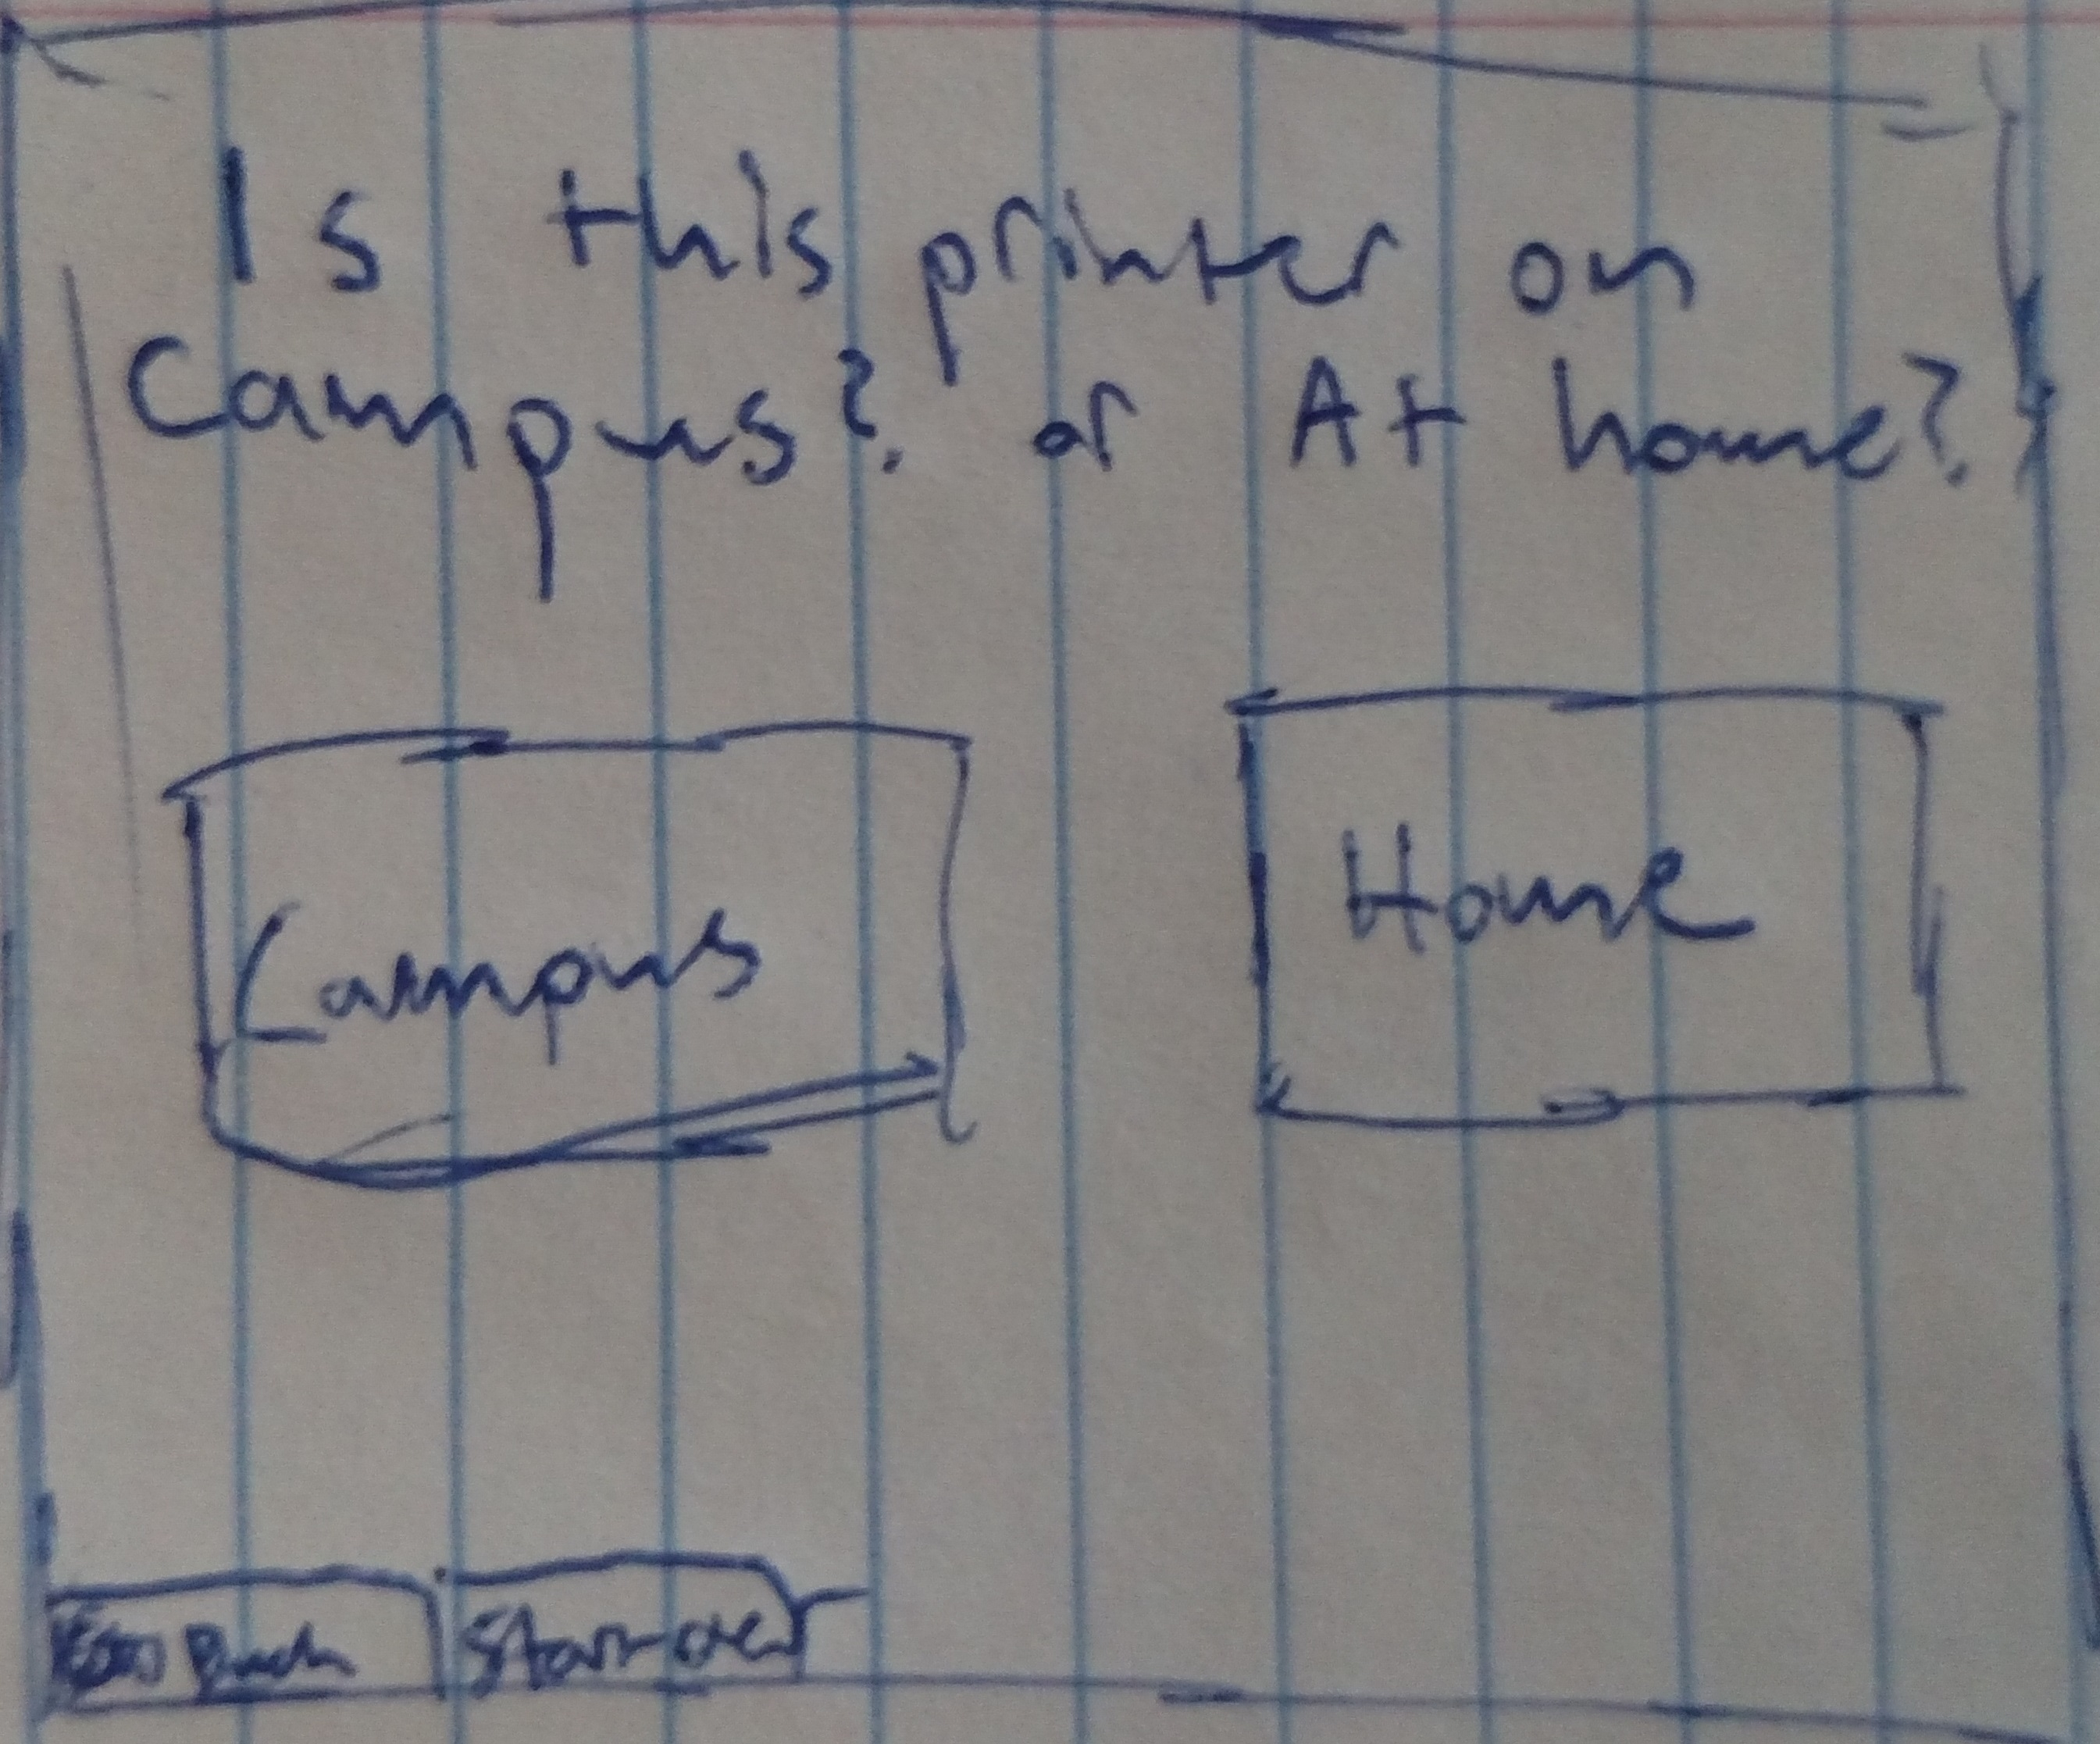
\includegraphics[scale=.075]{campus_or_home.jpg}
	\\After choosing that a printer is issue, the user is prompted with whether or not this is a personal printer or one that’s on campus. In this use case the user selects campus printer.
	\\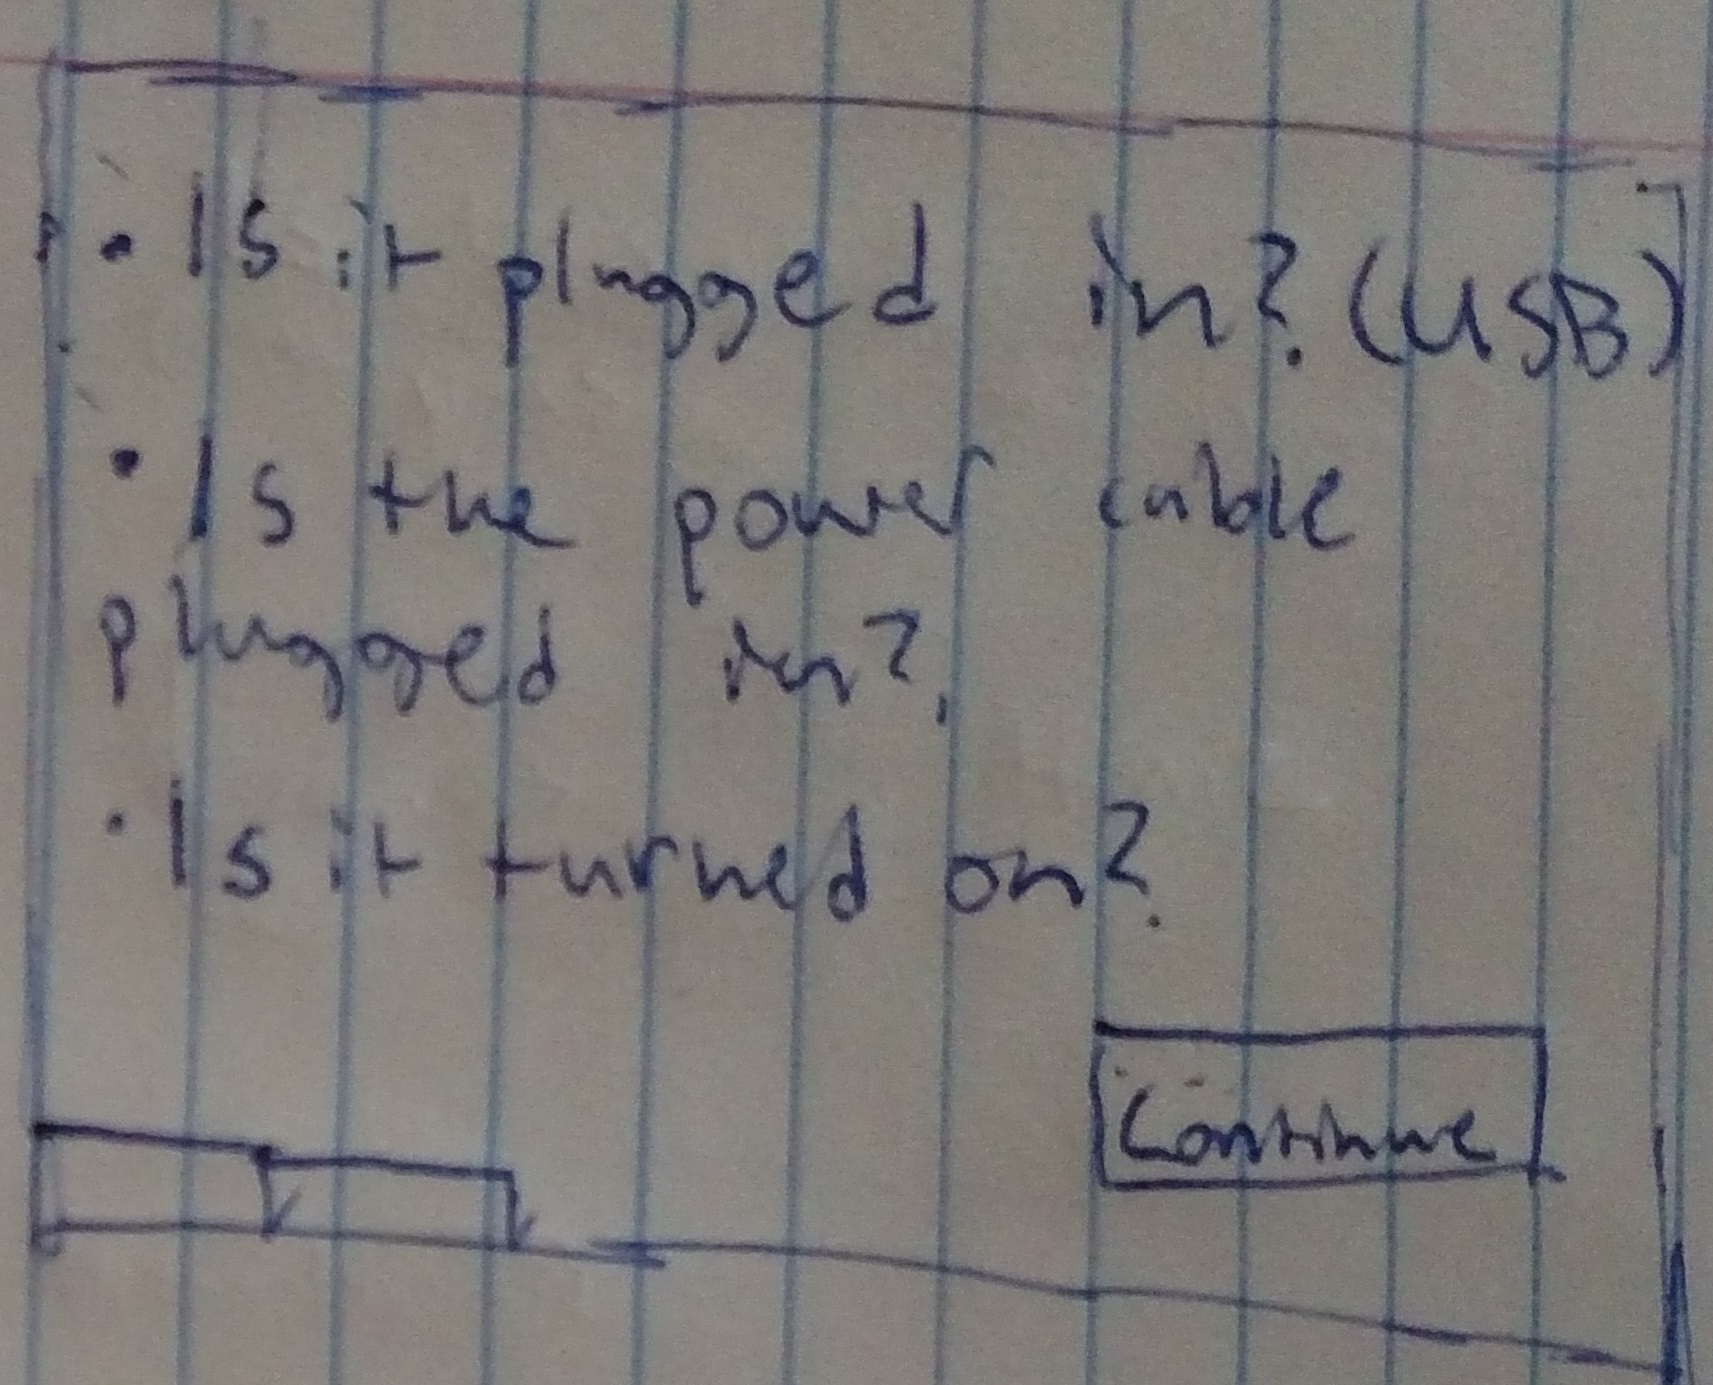
\includegraphics[scale=.075]{questions_1.jpg}
	\\Then the user is taken to a list of questions depending on their answer to the previous screen. The questions range from whether they have plugged in the power adapter, it’s turned on, and if the printer is plugged into the computer. If the user has verified the above, it is most likely indicating a malfunctioned driver.
	\\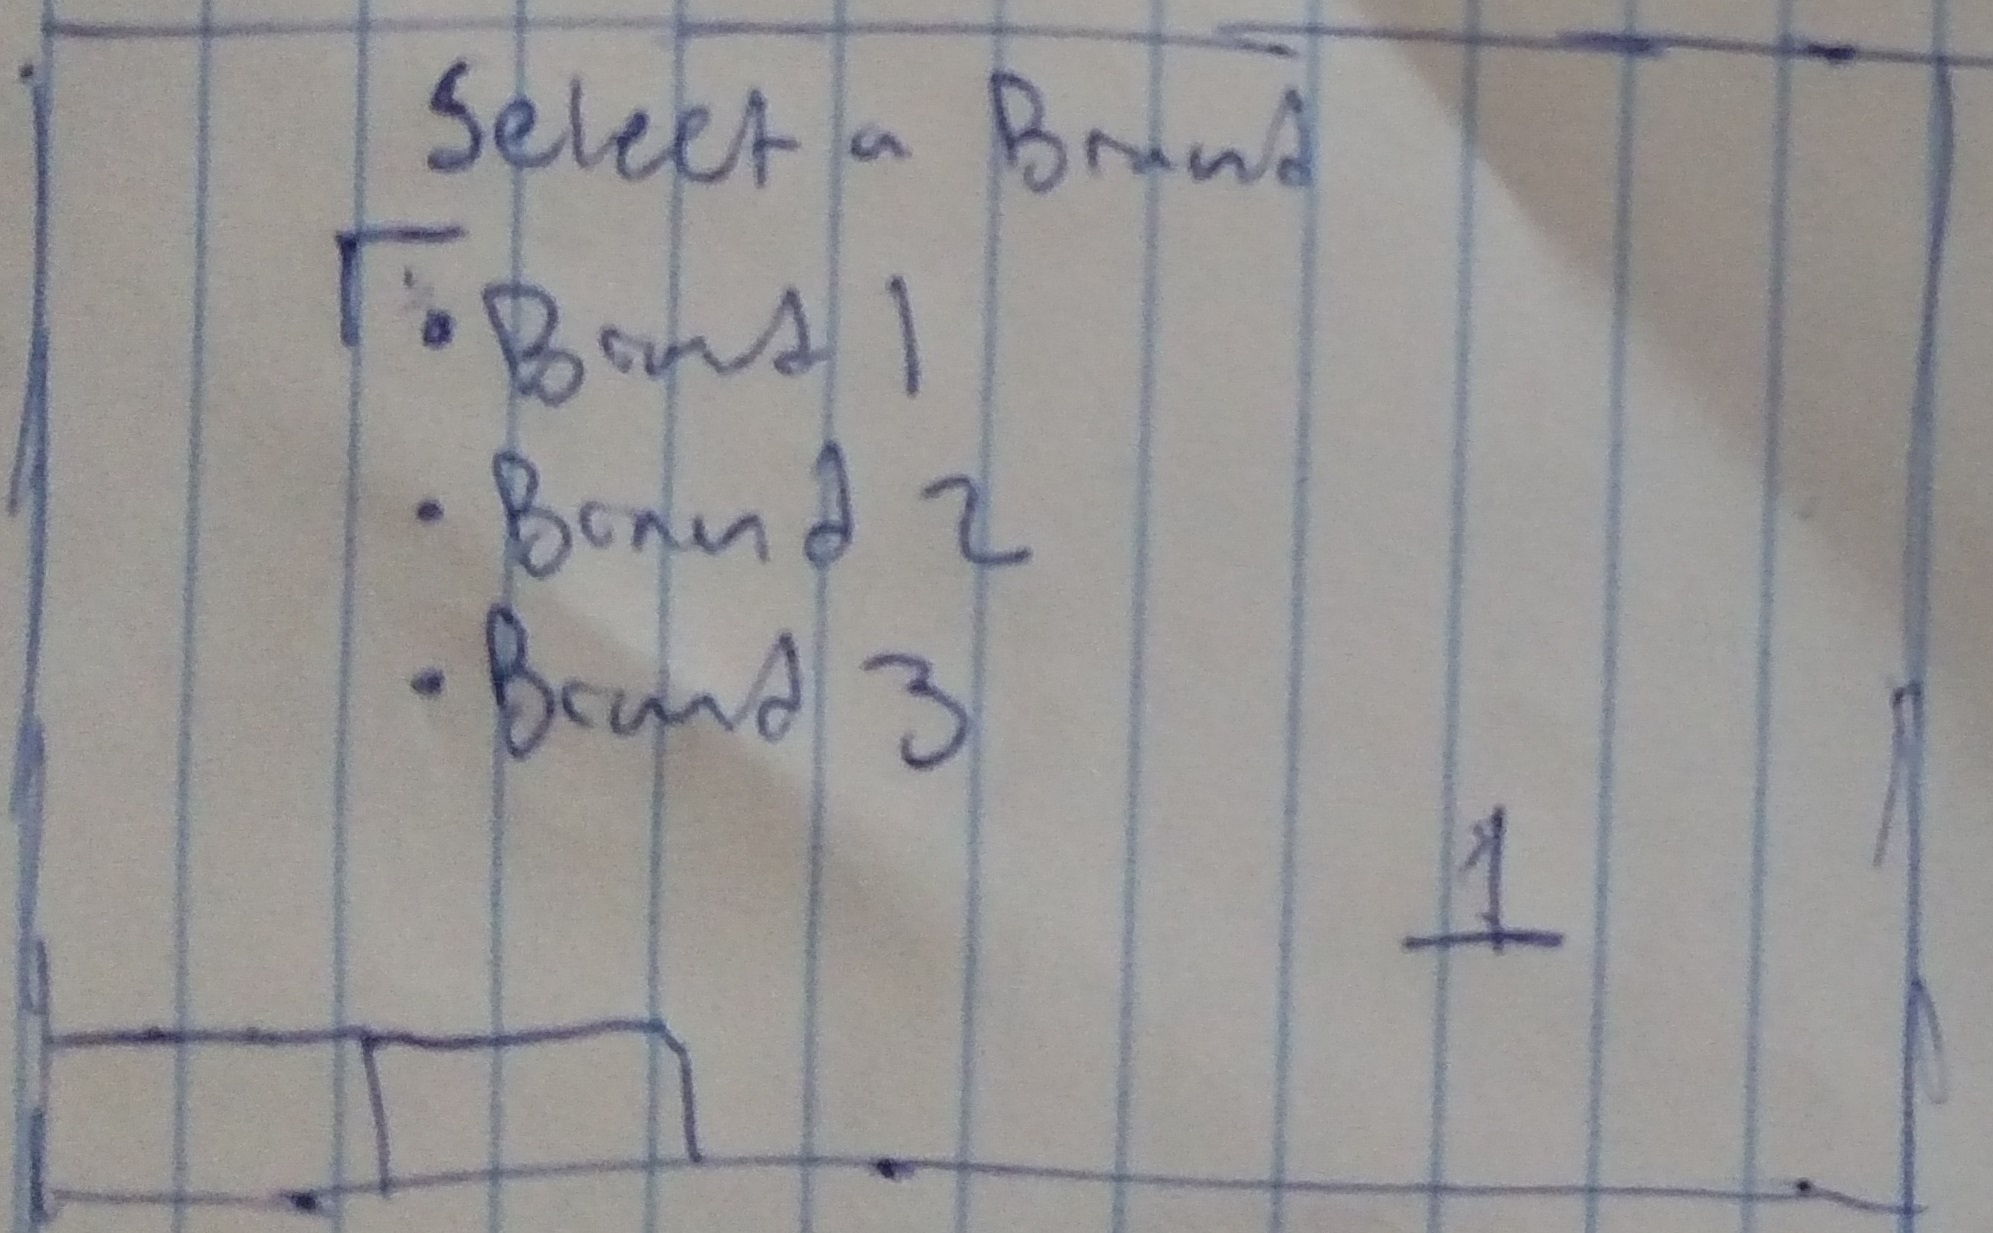
\includegraphics[scale=.075]{brands.jpg}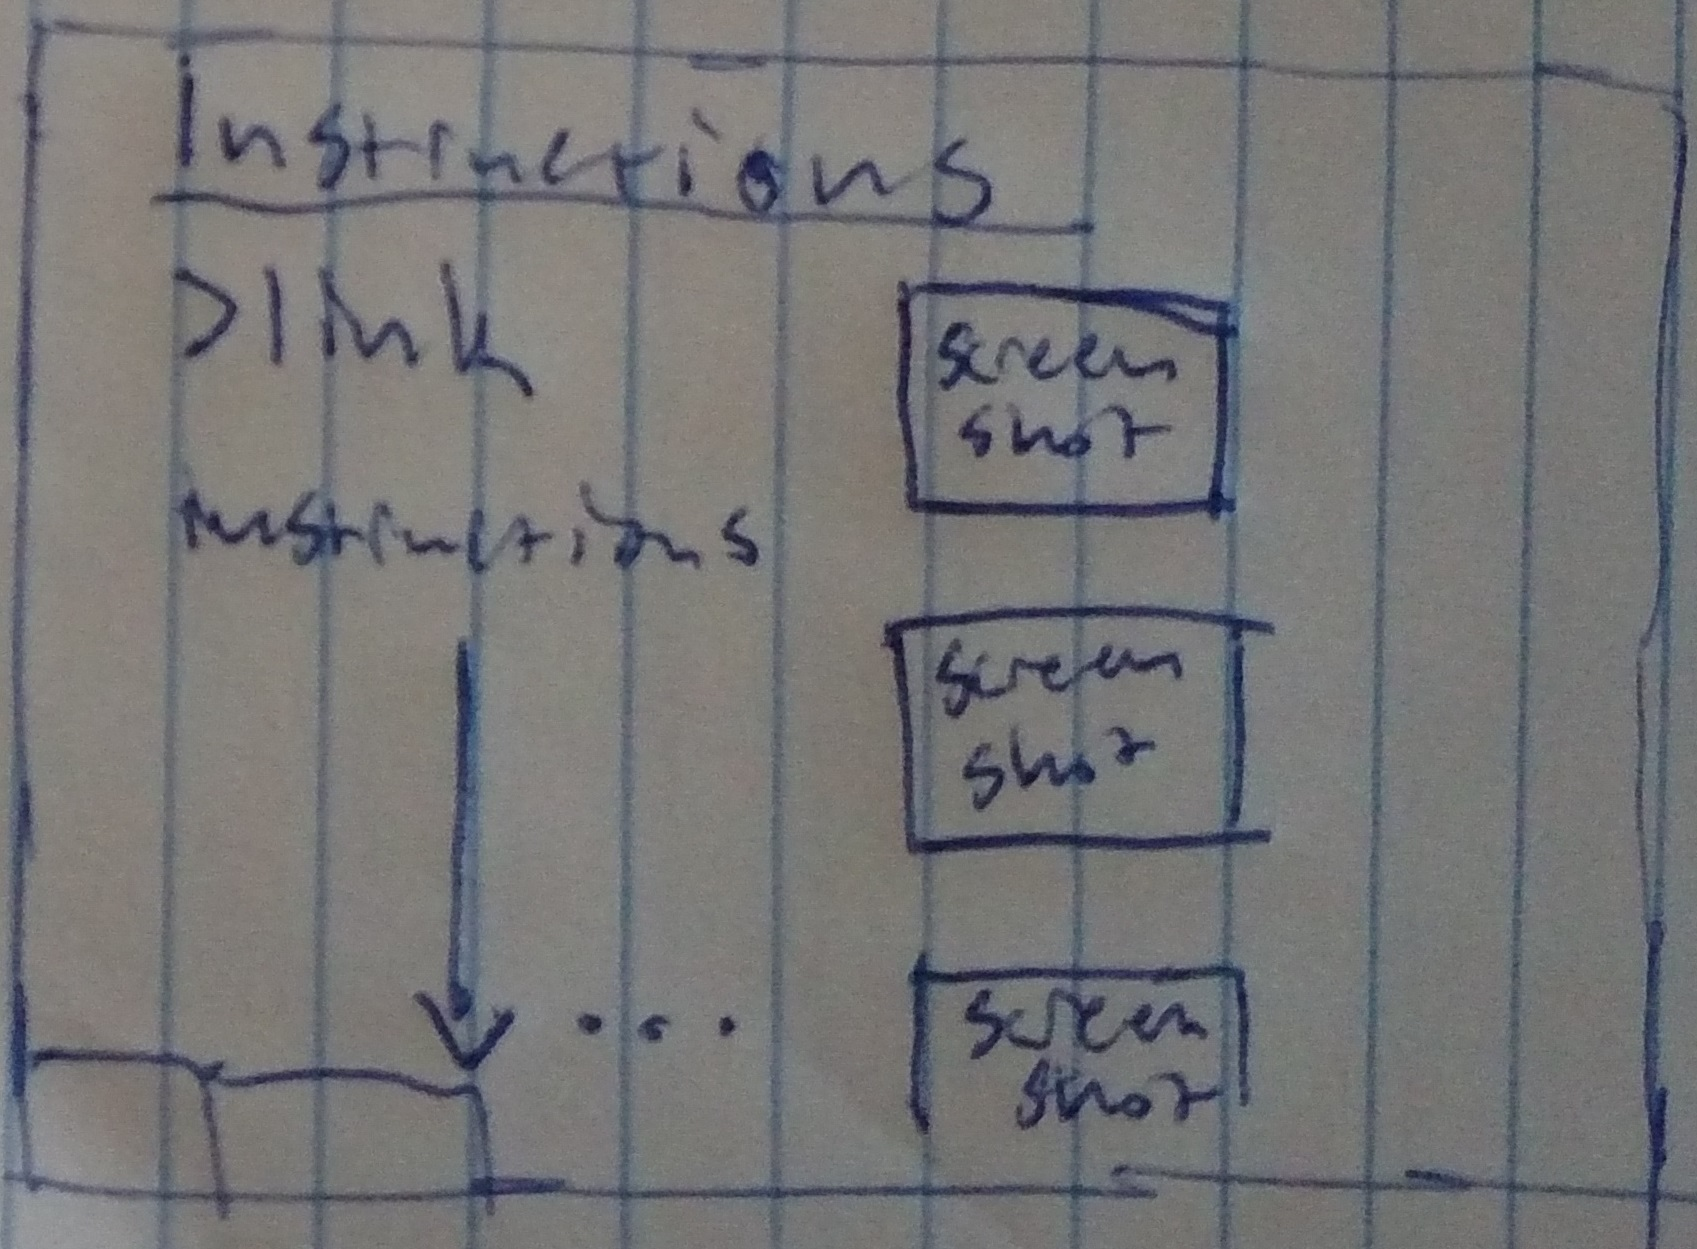
\includegraphics[scale=.075]{instructions.jpg}
	\\User then chooses the brand of their printer of a scrollable list and is given a link to the site, with instructions for how to download and install the driver.
	\\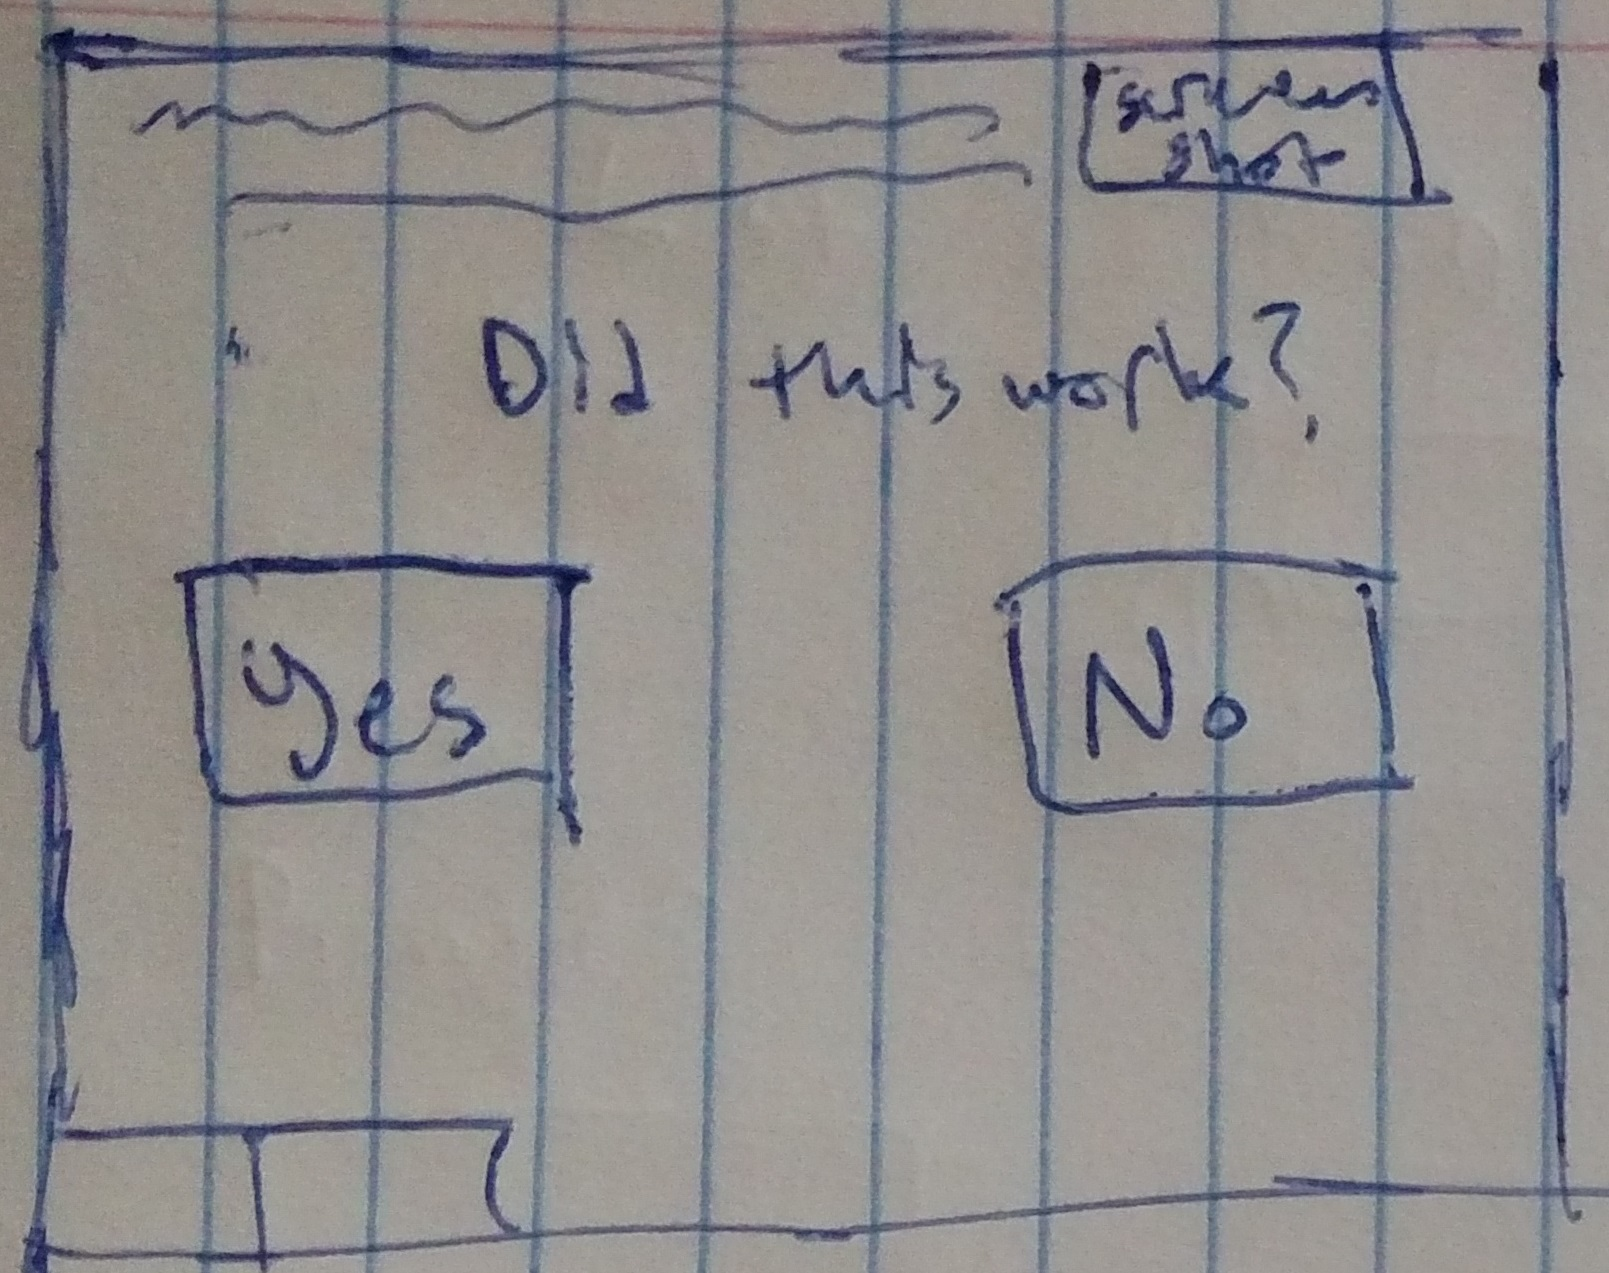
\includegraphics[scale=.075]{work.jpg} 
	\\User then chooses whether that worked or not it worked when they reach the bottom of the instructions. Success takes them back to the homescreen. If it failed, they are given the option to go to the windows troubleshooting site and then asked if they need help again. 
	\\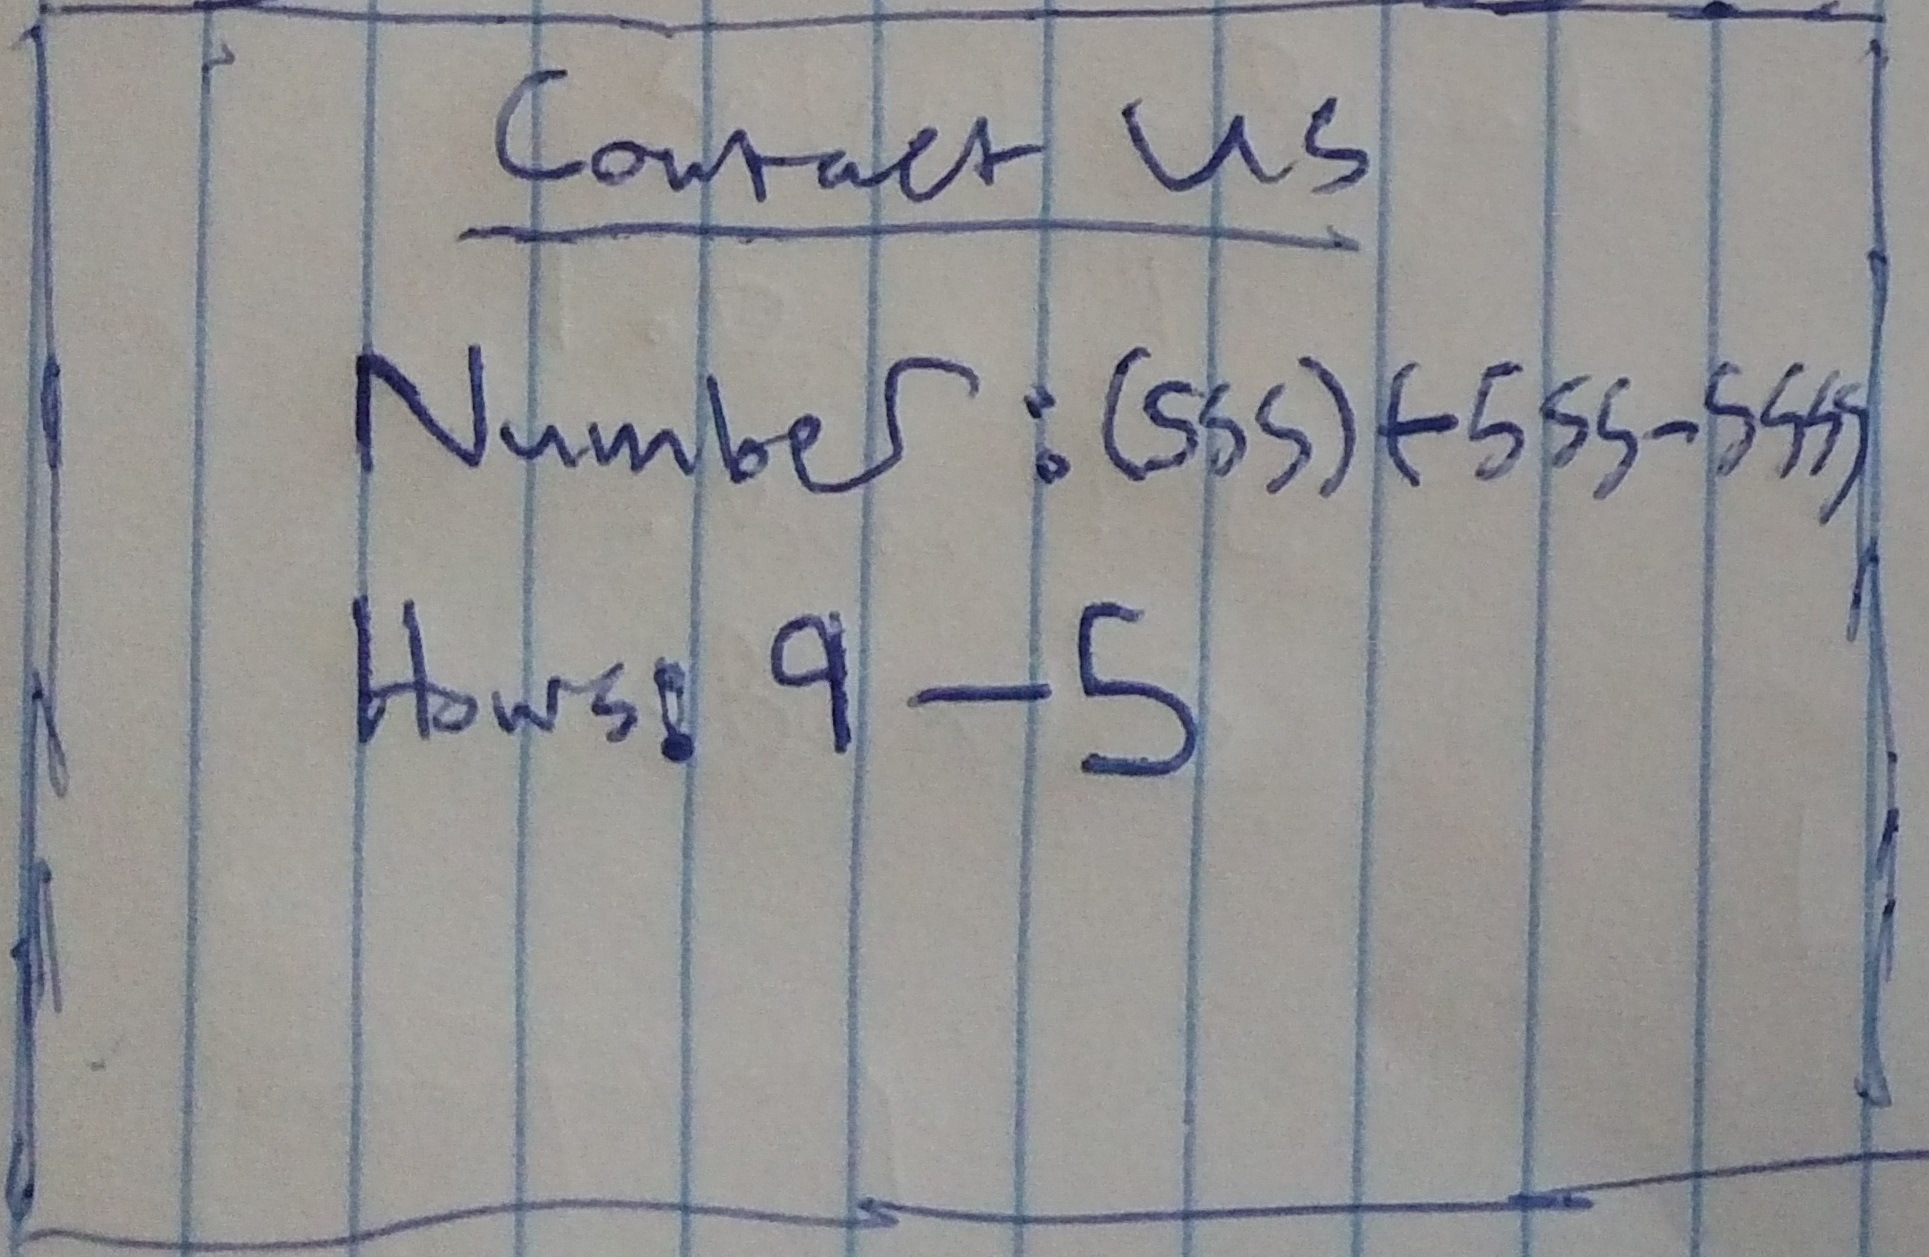
\includegraphics[scale=.075]{contact_us.jpg}
	\\If they choose the option saying that they found their answer then it returns to the homescreen. However, in this case the app gives them the number for tech support, alongside the hours since they still require assistance.  
	\\
\end{enumerate}	
\underline{\textbf{Class Diagram:}}
\\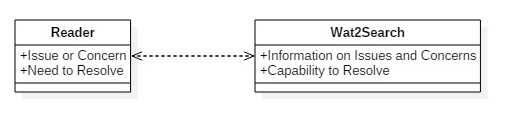
\includegraphics[scale=.75]{class_diagram.png}
\\This class diagram describes the relationship our prospective reader and our tool have: The reader has an issue/concern that they wish to address, and our tool is what can be used to address it, with the capability to resolve it; either through direct means and step-by-step guidance, or by informing the user of their situation and directing them where to go next when the situation is out of their scope.
\\\\\\\\
\\\\\\\\
\\\\\\\\
\\\\\\\\\\
\\\\\\\\\\\\\\\\\\\\\\
\underline{\textbf{Sequence Diagrams:}}
\\These sequence diagrams use the format of Use Case Design, where the user of our software (named as \textbf{Reader}), has a particular issue that they wish to resolve, and that after consulting our software, they are informed of what they need to do, depending on the level of difficulty of their task.
\\\\Use Case 1:
\\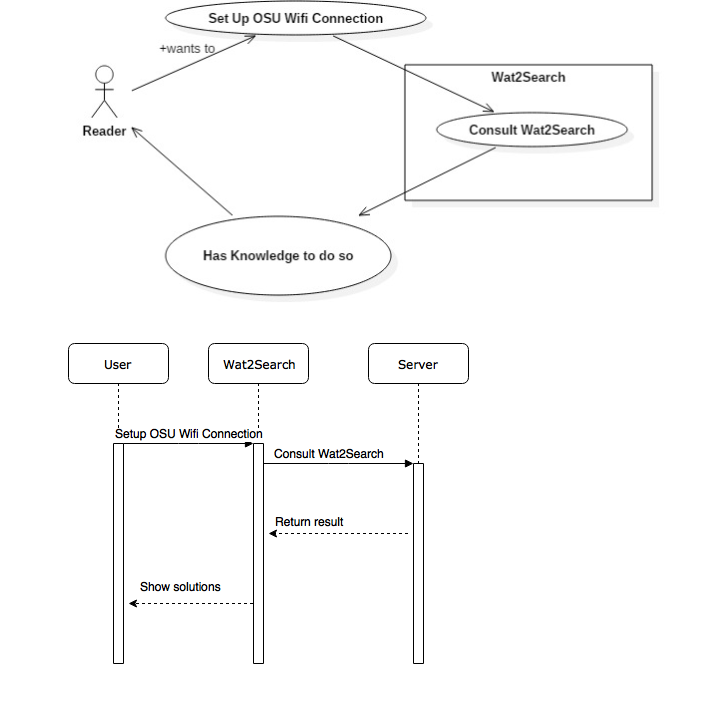
\includegraphics[scale=.75]{use_case1.png}
\\\\Use Case 2:
\\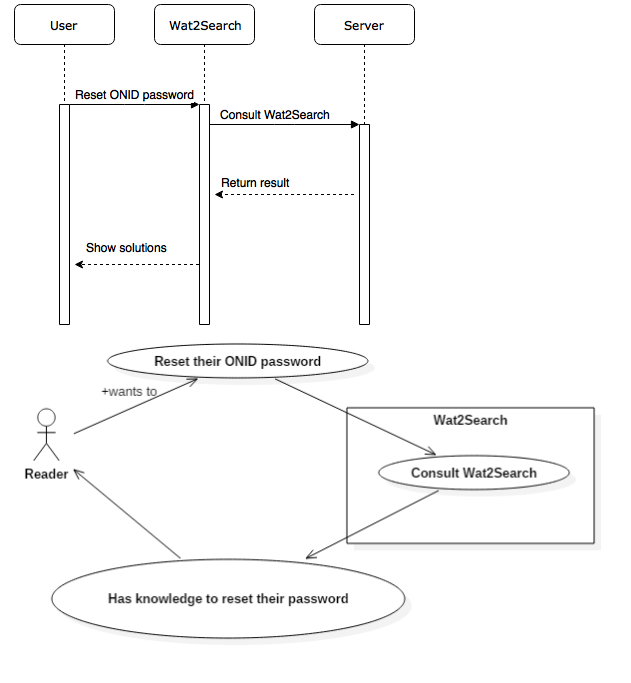
\includegraphics[scale=.75]{use_case2.png}
\\\\\\\\\\\\\\\\\\\\\\Use Case 3:
\\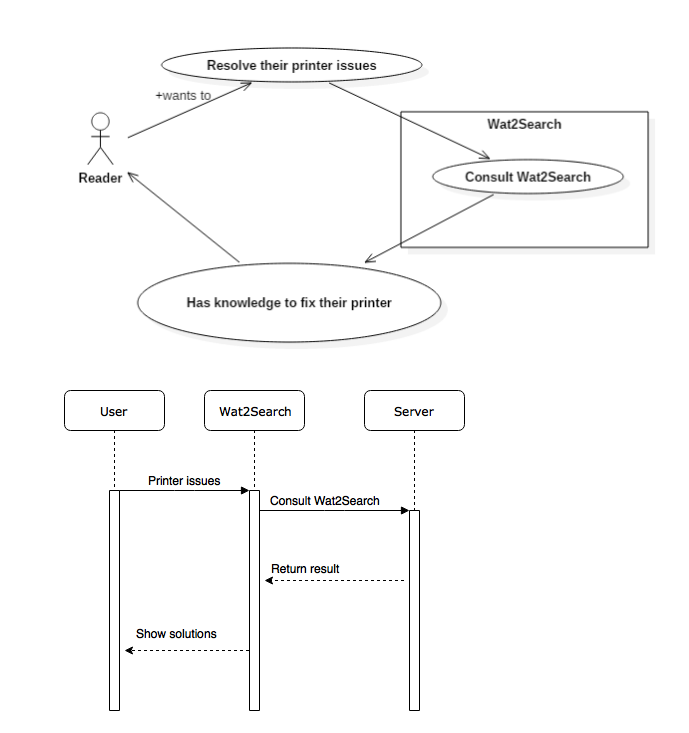
\includegraphics[scale=.75]{use_case3.png}
\\\\\\\\\\\\\\\\
\\\underline{\textbf{Meeting Report:}}
\\We scheduled to meet up Saturday at 1:00pm in the library to discuss goals for this project for this week as well as following weeks. This was our first formal, in person meeting. Everybody made it on time. We met in the first floor,sat around a table, and got a whiteboard with markers to mock up our ideas. Lauren had drawn the ui on her notebook earlier, which we are using as our basis. We decided to remove the search bar concept which was originally sketched, as users who struggle with technology might be intimidated by a list of multiple potential issues. We nailed down our six starting categories for the home screen as well as what the icons for them should be. Donghao brought up adding a router symbol for users who may not understand how networks work. For the placement of the program we decided that widget would be integrated into the user’s current window rather than taking them to a new tab or window. This allows for the user to more easily look up help without moving away from what they are looking at.

On the UI Robert did a mockup on the whiteboard of the homescreen categories being split into tiles that leads to questions for the users. That lead into questions we would pose for the user. For our prototype we went with about 3 common questions on each category as placeholders. 

We’ve kept in contact over Discord and assigned tasks based on voting on a poll. During this meeting at the library we also finalized who was doing what for the rest of this assignment.  Evan, Luke and Lauren added the user interface prototype mockups based on a powerpoint slide made by Robert. Each of us decided to take on two pages for each use case we made in the previous assignment. Evan did the meeting report for this week and converted this document to LaTex due to familiarity with the program from previous assignments.  Robert decided to write the class diagram since he has the best idea of how he wanted this program to be structured when he came up with the initial idea for Wat2Search. Luke and Dongao did the sequence diagrams, since they had an interest in UMLs.

During our meeting we also looked up different UML diagram creation programs, we decided on StarUML since it’s free and has a modern UI. We found that it could be exported to png and edited further in any painting program. It also runs on multiple operating systems so the Mac users in our group can use it too. Given the simplicity of our project we emailed the TA to see if a UML would be needed. Regardless, we are set up to make one if need be. 

Overall, we all got onto the same page and decided on tasks we were comfortable working on.  There was heavy involvement from everyone in the brainstorming process. We also got a good idea of what our limits are for this term, what problems we could solve for users in the scope of this class. We went on a basic structure and flow, something simple for any user in need of tech support. 




\end{document}
